\subsection*{Question 2.10}

We are to try out various numbers of hidden units in the neural
network. From figure \ref{fig:q210hidden} we see that using $260$
hidden units performs the best on the test data with $27.31\%$
error. The resulting decision boundaries can be seen in figure
\ref{fig:q210Nh260}. The boundary is rather complex due to the large
number of hidden units within the network. As another example figure
\ref{fig:q210Nh2} shows decision boundaries using only $2$ hidden
units. This results in a nearly linear boundary, due to the
inflexibility of using only $2$ hidden units. As opposed to $2$ and
$260$ hidden units, figure \ref{fig:q210Nh1000} shows the result of
using $1000$ hidden units. We now have a situation where we have low
misclassification rate on the training data scoring $22.00\%$ error,
but the model do not generalize very well resulting in $29.12\%$ on
the test data. From the figure it can be seen that the model tends
towards overfitting, by having more curvatures.

\begin{figure}[!htbp]
  \centering
  \subfloat[\label{subfig:q210Nh10}]{
  \begin{tabular}{|c|c|}
    \hline
    \multicolumn{2}{|c|}{Hidden units $= 10$} \\
    \hline
    Training error: 24.67\% & Test error: 29.38\% \\
    \hline
  \end{tabular}
  }
  \subfloat[\label{subfig:q210Nh30}]{
    \begin{tabular}{|c|c|}
      \hline
      \multicolumn{2}{|c|}{Hidden units $= 30$} \\
      \hline
      Training error: 25.33\% & Test error: 28.75\% \\
      \hline
    \end{tabular}
  } \\
  \subfloat[\label{subfig:q210Nh60}]{
    \begin{tabular}{|c|c|}
      \hline
      \multicolumn{2}{|c|}{Hidden units $= 60$} \\
      \hline
      Training error: 23.33\% & Test error: 28.00\% \\
      \hline
    \end{tabular}
  } 
  \subfloat[\label{subfig:q210Nh100}]{
    \begin{tabular}{|c|c|}
      \hline
      \multicolumn{2}{|c|}{Hidden units $= 100$} \\
      \hline
      Training error: 22.67\% & Test error: 28.31\% \\
      \hline
    \end{tabular}
  } \\
  \subfloat[\label{subfig:q210Nh130}]{
    \begin{tabular}{|c|c|}
      \hline
      \multicolumn{2}{|c|}{Hidden units $= 130$} \\
      \hline
      Training error: 22.67\% & Test error: 28.12\% \\
      \hline
    \end{tabular}
  } 
  \subfloat[\label{subfig:q210Nh200}]{
    \begin{tabular}{|c|c|}
      \hline
      \multicolumn{2}{|c|}{Hidden units $= 200$} \\
      \hline
      Training error: 23.33\% & Test error: 27.88\% \\
      \hline
    \end{tabular}
  } \\
  \subfloat[\label{subfig:q210Nh260}]{
    \begin{tabular}{|c|c|}
      \hline
      \multicolumn{2}{|c|}{Hidden units $= 260$} \\
      \hline
      Training error: 22.67\% & Test error: \textbf{27.31\%} \\
      \hline
    \end{tabular}
  } 
  \subfloat[\label{subfig:q210Nh300}]{
    \begin{tabular}{|c|c|}
      \hline
      \multicolumn{2}{|c|}{Hidden units $= 300$} \\
      \hline
      Training error: 24.00\% & Test error: 27.81\% \\
      \hline
    \end{tabular}
  } \\
  \subfloat[\label{subfig:q210Nh500}]{
    \begin{tabular}{|c|c|}
      \hline
      \multicolumn{2}{|c|}{Hidden units $= 500$} \\
      \hline
      Training error: 22.67\% & Test error: 29.31\% \\
      \hline
    \end{tabular}
  } 
  \subfloat[\label{subfig:q210Nh1000}]{
    \begin{tabular}{|c|c|}
      \hline
      \multicolumn{2}{|c|}{Hidden units $= 1000$} \\
      \hline
      Training error: \textbf{22.00\%} & Test error: 29.12\% \\
      \hline
    \end{tabular}
  }
  \caption{Show the result of running the neural network with various
    numbers of hidden units.}
  \label{fig:q210hidden}
\end{figure}

\begin{figure}[!htbp]
  \centering
  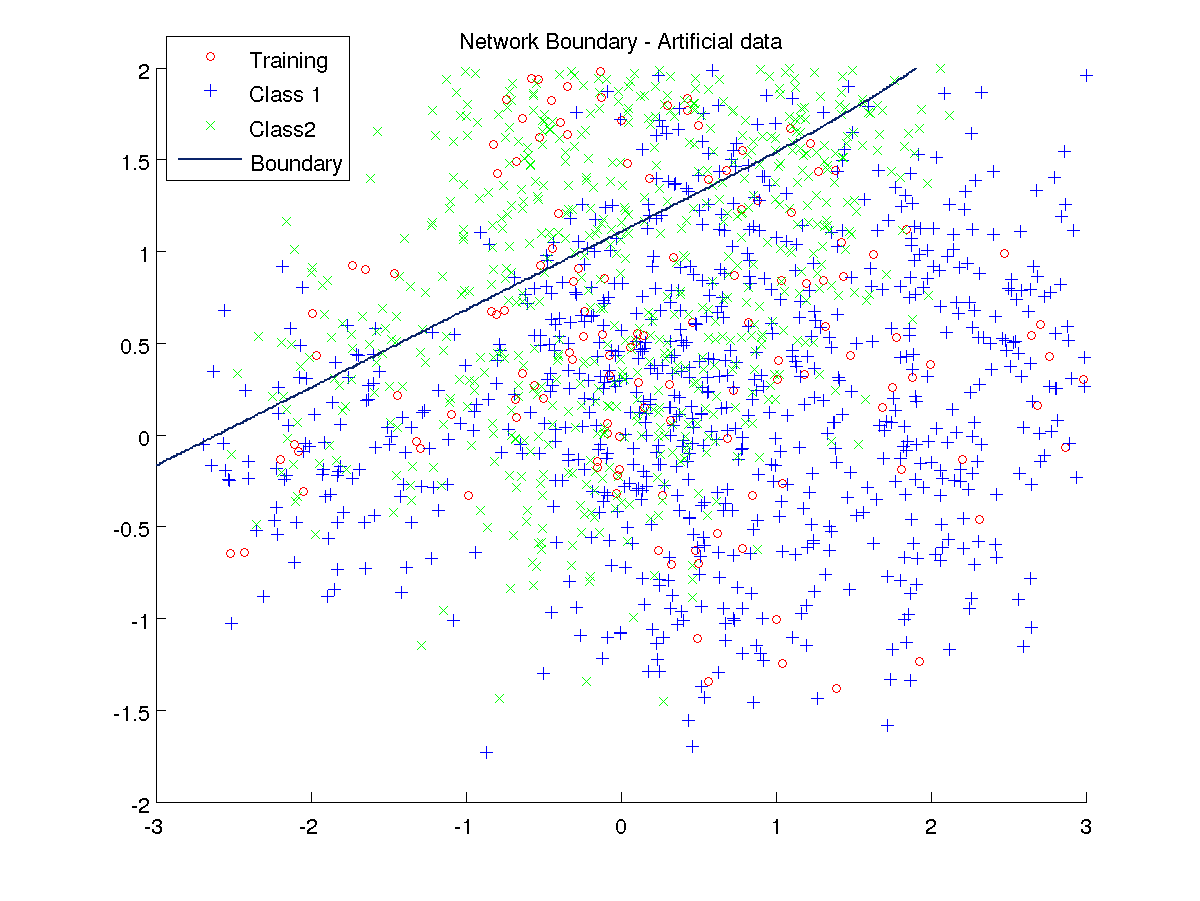
\includegraphics[width=0.6\textwidth]{./images/q210a_Nh2}
  \caption{Show neural network using $2$ hidden units, resulting in a
    nearly linear decision boundary.}
  \label{fig:q210Nh2}
\end{figure}

\begin{figure}[!htbp]
  \centering
  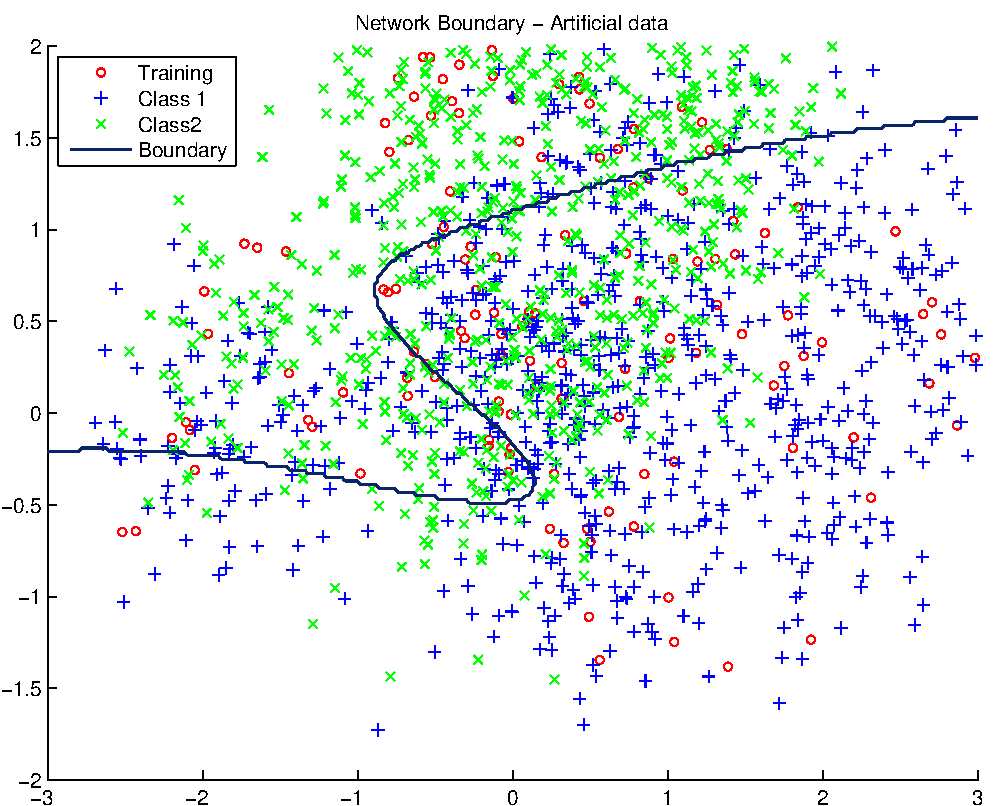
\includegraphics[width=0.6\textwidth]{./images/q210a_Nh260}
  \caption{Show neural network using $260$ hidden units, resulting in
    a rather complex decision boundary, but not overfitted.}
  \label{fig:q210Nh260}
\end{figure}

\begin{figure}[!htbp]
  \centering
  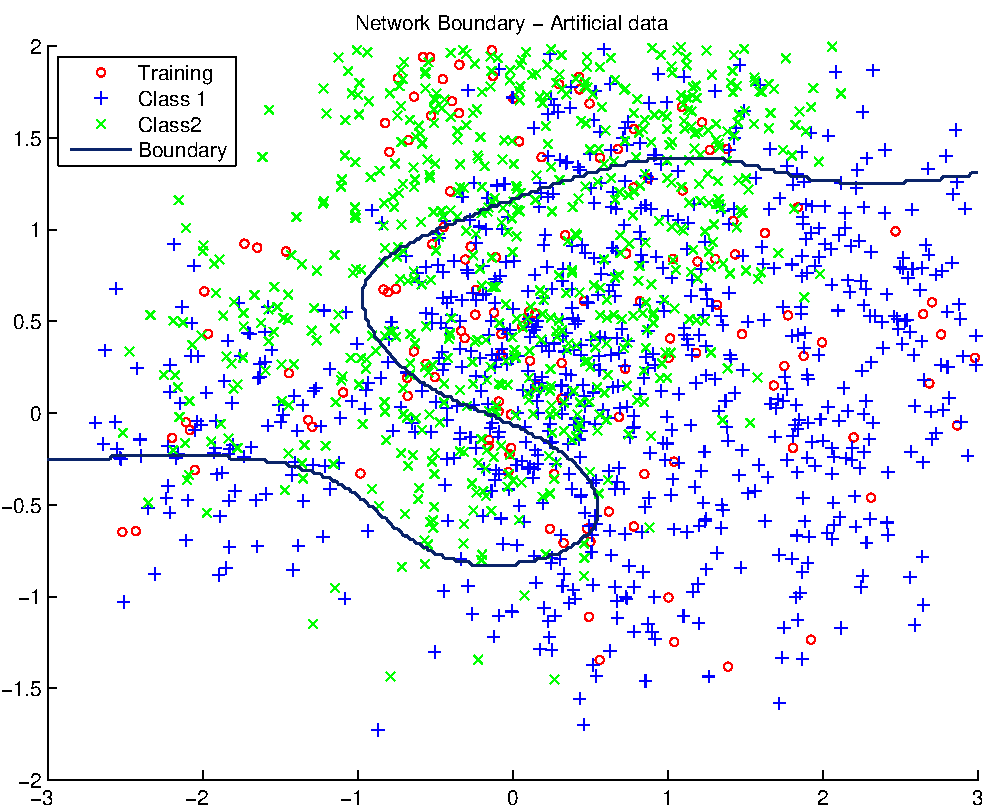
\includegraphics[width=0.6\textwidth]{./images/q210a_Nh1000}
  \caption{Show neural network using $1000$ hidden units, resulting in
    a complex decision boundary with many curvatures, this seems too
    overfitted for the data.}
  \label{fig:q210Nh1000}
\end{figure}

Our results suggests that using a neural network model with
intermediate complexity results in the best generalization. Choosing
$260$ hidden units performs the best.

We are now to experiment with using regulization to control the
complexity of the model using a fixed number of hidden units. The
result of the experiments can be seen in figure
\ref{fig:q210bregulization}. The figure \ref{fig:q210breg2} show the
plot of \ref{subfig:q210btrain}, the result suffers from overfitting
it produces the lowest training error, but the test error suffer from
the lack of generalization. Using $0.025119$ as regulization
coefficient produces the most general model, this produces a near
linear decision boundary which can be seen in \ref{fig:q210breg3}. A
to simple model is shown in figure \ref{fig:q210breg5}, this is using
$6.309573$ as regulization coefficient, this results in a total linear
model due to the regulization of the weight parameters in the model. A
graph of the error values can be seen in figure \ref{fig:q210berror}
bottom.

\begin{figure}[!htbp]
  \centering
  \subfloat[\label{subfig:q210btrain}]{
    \begin{tabular}{|c|c|}
      \hline
      \multicolumn{2}{|c|}{Regulization coefficient $= 0.001585$} \\
      \hline
      Training error: \textbf{26.00\%} & Test error: 29.38\% \\
      \hline
    \end{tabular}
  }
  \subfloat[\label{subfig:q210btest}]{
  \begin{tabular}{|c|c|}
    \hline
      \multicolumn{2}{|c|}{Regulization coefficient $= 0.025119$} \\
      \hline
      Training error: 27.00\% & Test error: \textbf{28.25\%} \\
      \hline
    \end{tabular}
  }
  \caption{\ref{subfig:q210btrain} shows the best result on training
    data, \ref{subfig:q210btest} shows the best result on test data}
  \label{fig:q210bregulization}
\end{figure}

\begin{figure}[!htbp]
  \centering
  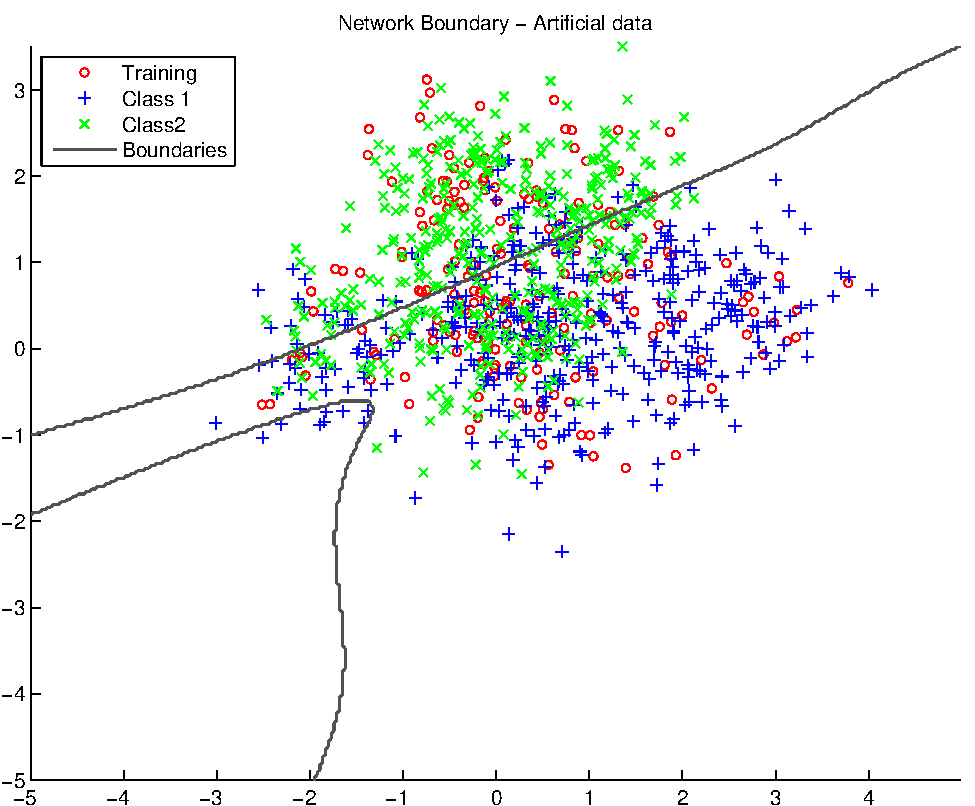
\includegraphics[width=0.6\textwidth]{./images/q210b_reg2}
  \caption{Show neural network using regulization coefficient at $0.001585$, resulting in
    a complex decision boundary, this seems to tends towards overfitted.}
  \label{fig:q210breg2}
\end{figure}

\begin{figure}[!htbp]
  \centering
  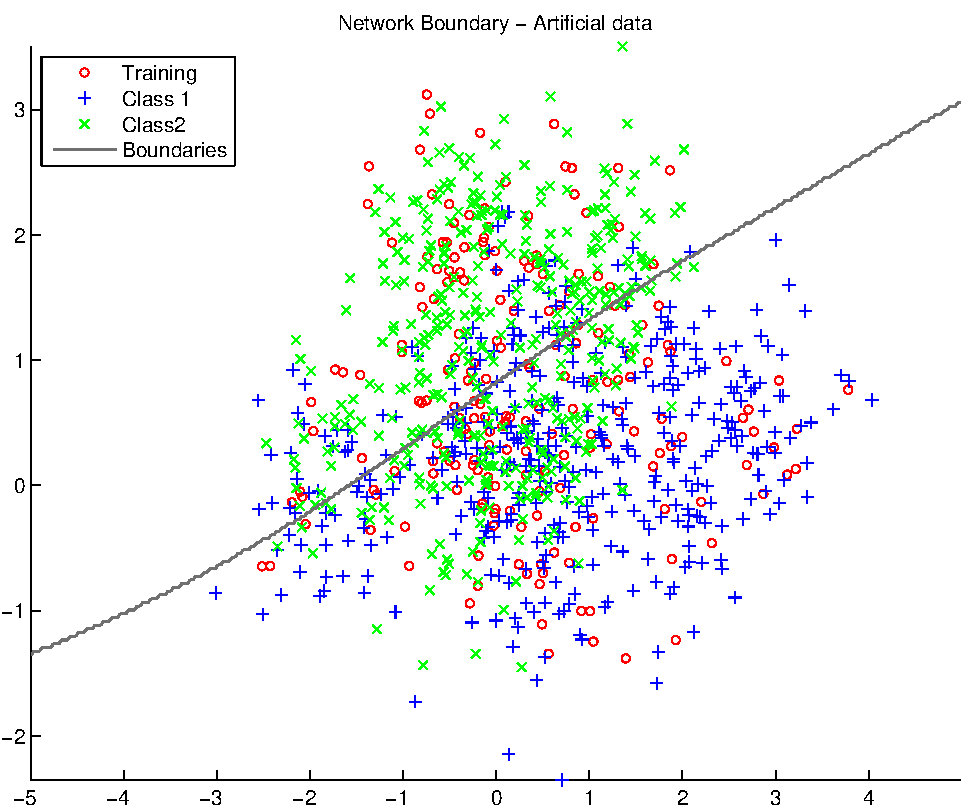
\includegraphics[width=0.6\textwidth]{./images/q210b_reg3}
  \caption{Show neural network using regulization coefficient at $0.025119$, resulting in
    a simple near linear decision boundary, not overfitted.}
  \label{fig:q210breg3}
\end{figure}

\begin{figure}[!htbp]
  \centering
  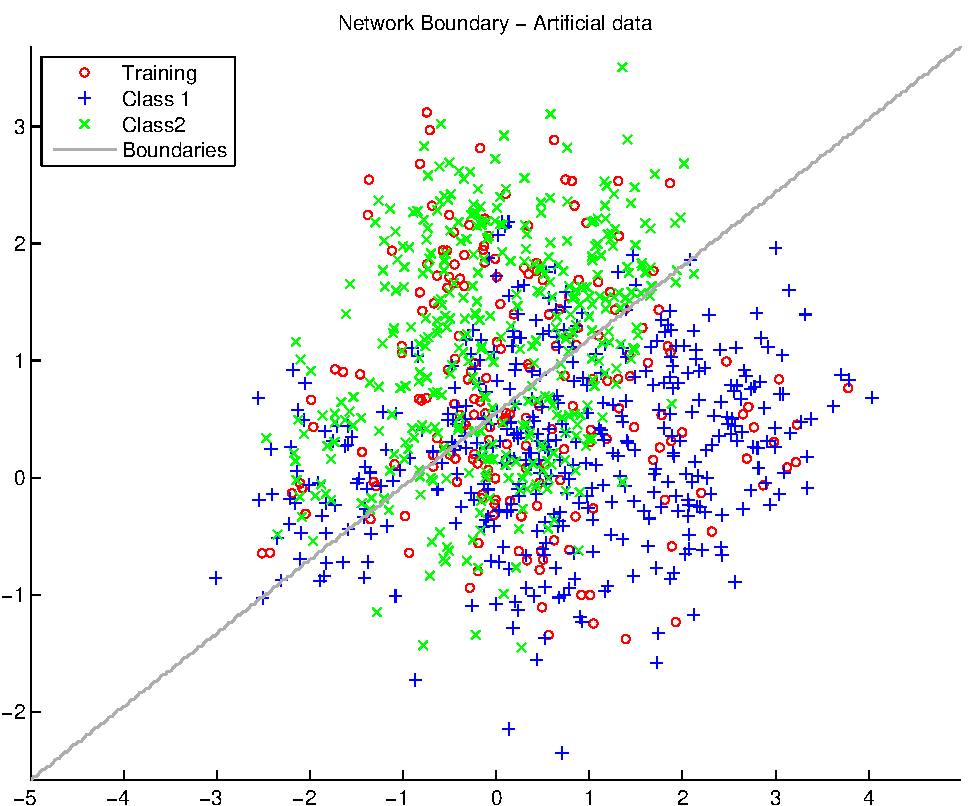
\includegraphics[width=0.6\textwidth]{./images/q210b_reg5}
  \caption{Show neural network using regulization coefficient at $6.309573$, resulting in
    a linear decision boundary.}
  \label{fig:q210breg5}
\end{figure}

\begin{figure}[!htbp]
  \centering
  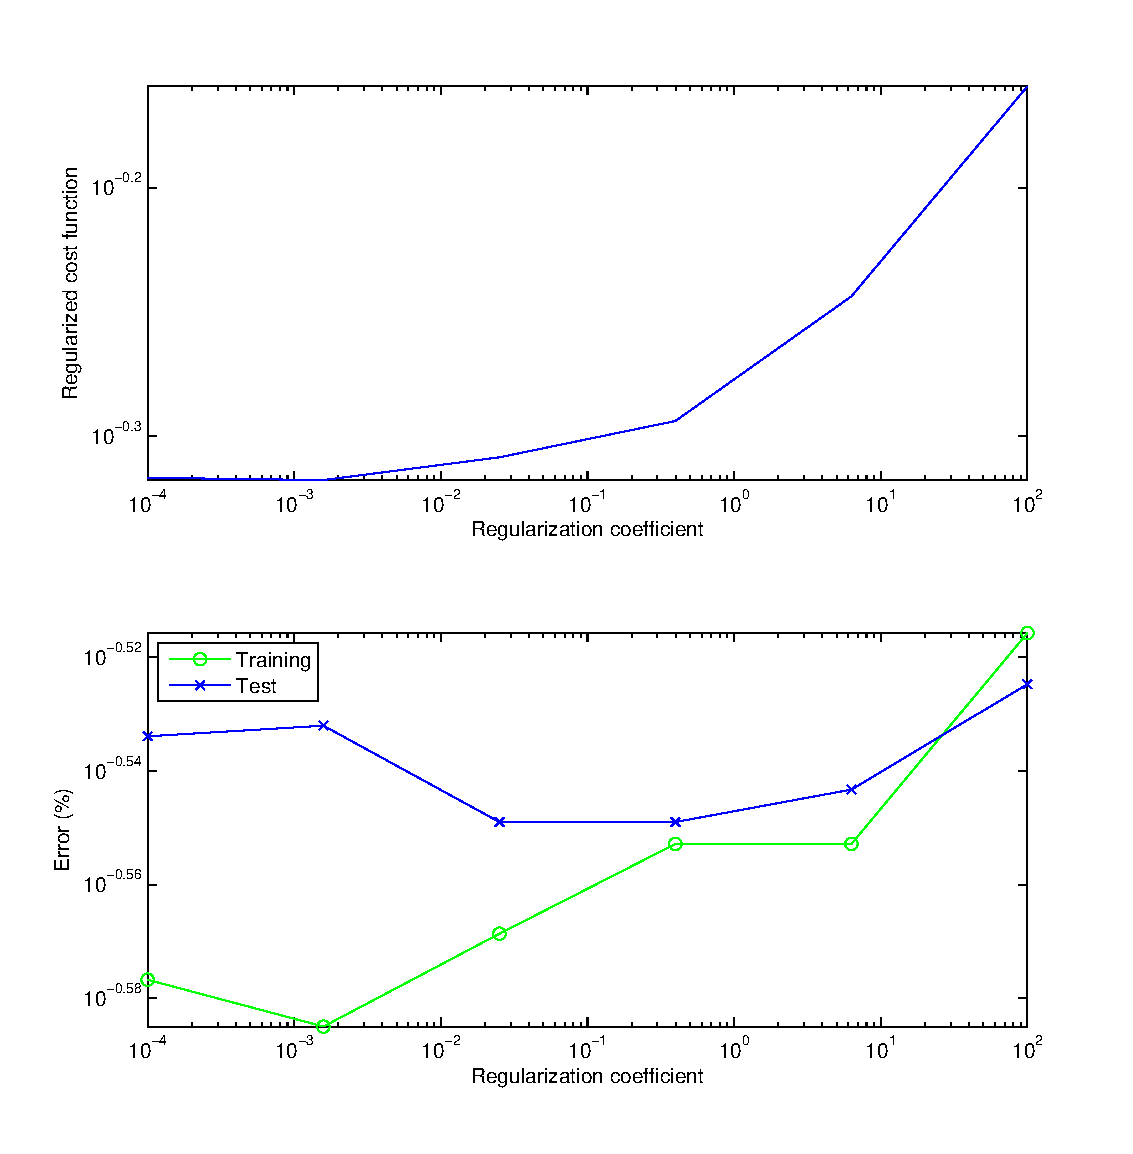
\includegraphics[width=0.8\textwidth]{./images/q210b_error}
  \caption{Shows error of training and test data in relation to the
    regulization coefficient. Also shows the regulized cost function
    in relation to the regulization coefficient.}
  \label{fig:q210berror}
\end{figure}
